%* 
%* ------------------------------------------------------------------
%* Model Railroad System by Deepwoods Software
%* ------------------------------------------------------------------
%* AddingNotes.tex - Adding notes
%* Created by Robert Heller on Tue Mar  5 08:40:22 2002
%* ------------------------------------------------------------------
%* Modification History: $Log$
%* Modification History: Revision 1.2  2004/04/14 23:22:17  heller
%* Modification History: Updated documentation.
%* Modification History:
%* Modification History: Revision 1.1  2002/11/09 21:21:07  heller
%* Modification History: Time Table User Manual
%* Modification History:
%* ------------------------------------------------------------------
%* Contents:
%* ------------------------------------------------------------------
%*  
%*     Model RR System, Version 2
%*     Copyright (C) 1994-2002  Robert Heller D/B/A Deepwoods Software
%* 			51 Locke Hill Road
%* 			Wendell, MA 01379-9728
%* 
%*     This program is free software; you can redistribute it and/or modify
%*     it under the terms of the GNU General Public License as published by
%*     the Free Software Foundation; either version 2 of the License, or
%*     (at your option) any later version.
%* 
%*     This program is distributed in the hope that it will be useful,
%*     but WITHOUT ANY WARRANTY; without even the implied warranty of
%*     MERCHANTABILITY or FITNESS FOR A PARTICULAR PURPOSE.  See the
%*     GNU General Public License for more details.
%* 
%*     You should have received a copy of the GNU General Public License
%*     along with this program; if not, write to the Free Software
%*     Foundation, Inc., 675 Mass Ave, Cambridge, MA 02139, USA.
%* 
%*  
%* 

\chapter{Adding, Editing, Etc. Notes}
\label{chapt:AddingNotes}

The {\tt Notes} menu manages the notes associated with a time table. 
These notes identify special conditions and situations, such as time
table variations, such as ``Sunday and Holiday'' schedules, meets, and
so on.

\section{View All Notes item}

The ``View All Notes'' menu item displays all notes currently defined. 
Each note is numbered.  A ``View All Notes'' pop-up is displayed, as
shown in Figure~\ref{fig:viewAllNotes}.

\begin{figure}
\begin{centering}
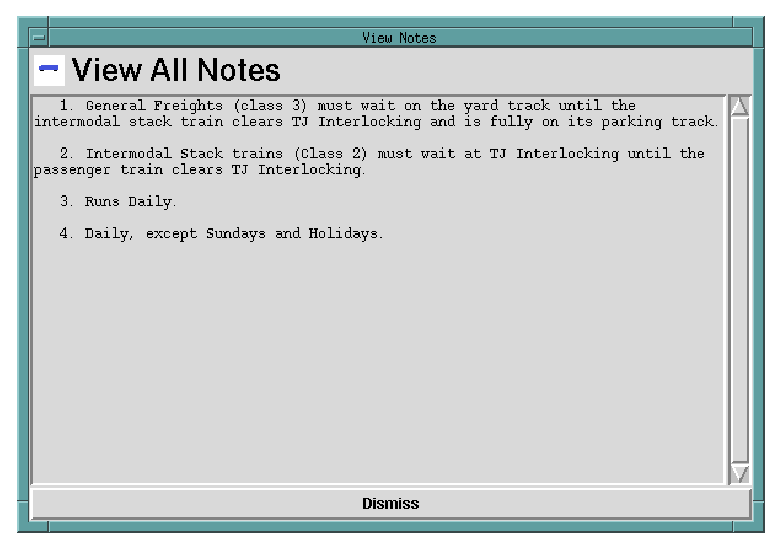
\epsfig{file=TimeTable/viewAllNotes.ps}\\
\caption{View All Notes pop-up.}
\label{fig:viewAllNotes}
\end{centering}
\end{figure}

\section{Create New Note item}
\label{sec:createNewNote}

\begin{figure}[h]
\begin{centering}
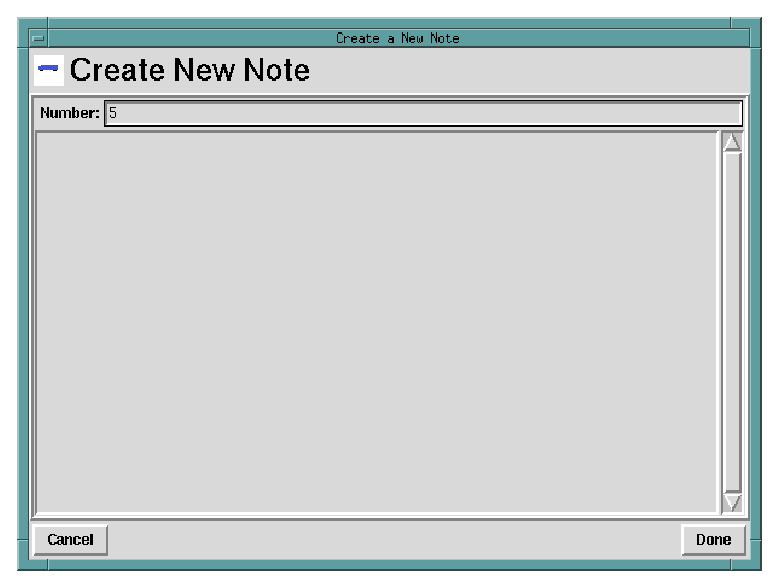
\epsfig{file=TimeTable/createNewNote.ps}\\
\caption{Create New Note dialog box.}
\label{fig:createNewNote}
\end{centering}
\end{figure} The ``Create New Note'' menu item is used to create a new
note.  The ``Create New Note'' dialog is displayed, as shown in
Figure~\ref{fig:createNewNote}.  This dialog box displays the next
available note number as a text area to enter the note in\footnote{The
note text is assumed to be \LaTeX\ code.  Normally, you can just enter
plain text, but certain characters are considered {\em spedial} to
\TeX\ and \LaTeX.  These include \%, \$, \&, \#. These characters can
be preceded with a backslash character to escape them.  On the other
hand you can include custom \LaTeX\ code to control the formatting of
your notes.}. 



\section{Delete Note item} 

The ``Delete Note'' menu item deletes a selected note.  You can only
delete notes that are not attached to a train (see
Sections~\ref{sect:addntotr} and \ref{sect:addntotrsta}).  The ``Delete
Note'' dialog box, show in Figure~\ref{fig:deleteNote}, is popped up.

\begin{figure}
\begin{centering}
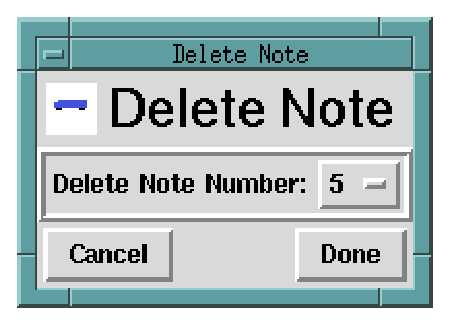
\epsfig{file=TimeTable/deleteNote.ps}\\
\caption{Delete Note dialog box.}
\label{fig:deleteNote}
\end{centering}
\end{figure}

\section{Edit Note item} 

\begin{figure}
\begin{centering}
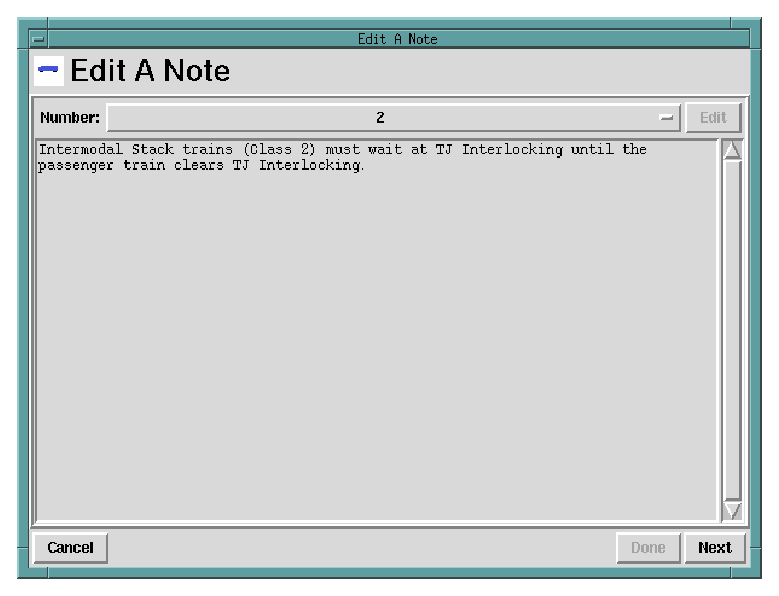
\epsfig{file=TimeTable/editNote.ps}\\
\caption{Edit Note dialog box.}
\label{fig:editNote}
\end{centering}
\end{figure} The ``Edit Note'' menu item edits a selected note. The
``Edit Note'' dialog box, show in Figure~\ref{fig:editNote}, is popped
up\footnote{See Section~\ref{sec:createNewNote}.}.



\section{Add Note To Train item} 
\label{sect:addntotr}

The ``Add Note To Train'' menu item adds a note to a train.  The note is
presumed to apply to the train as a whole, such as scheduling
restrictions, etc.  The ``Add Note To Train'' dialog box is displayed,
as shown in Figure~\ref{fig:addNoteToTrain}.

\begin{figure}
\begin{centering}
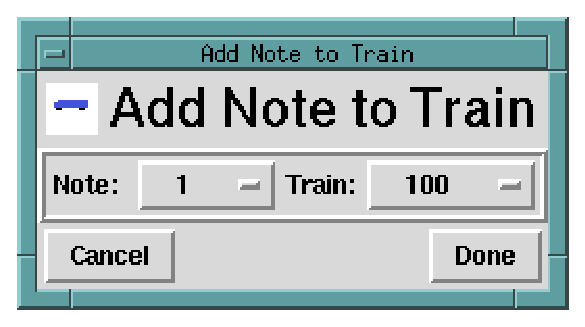
\epsfig{file=TimeTable/addNoteToTrain.ps}\\
\caption{Add Note To Train dialog box.}
\label{fig:addNoteToTrain}
\end{centering}
\end{figure}

\section{Add Note To Train at Station item}
\label{sect:addntotrsta}

The ``Add Note To Train at Station'' menu item adds a note to a train
at a specific station.  The note is presumed to apply to the train as
it is at the specified station, such as a meet or schedule switching
operations.  The ``Add Note To Train at Station'' dialog boxes are
displayed, as shown in Figures~\ref{fig:addNoteToTrainAtStation1} and
\ref{fig:addNoteToTrainAtStation2}.

\begin{figure} 
\begin{centering} 
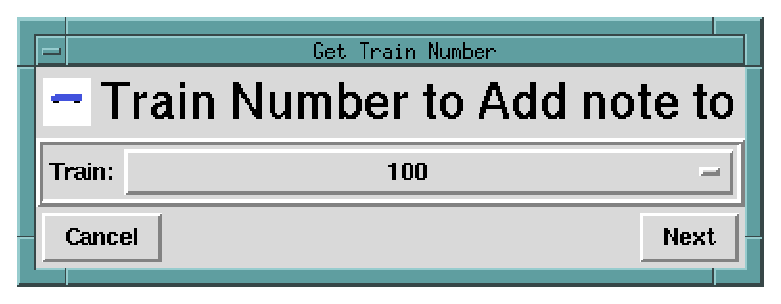
\epsfig{file=TimeTable/addNoteToTrainAtStation1.ps}\\
\caption{Add Note To Train at Station first dialog box.} 
\label{fig:addNoteToTrainAtStation1}
\end{centering} 
\end{figure}

\begin{figure} 
\begin{centering} 
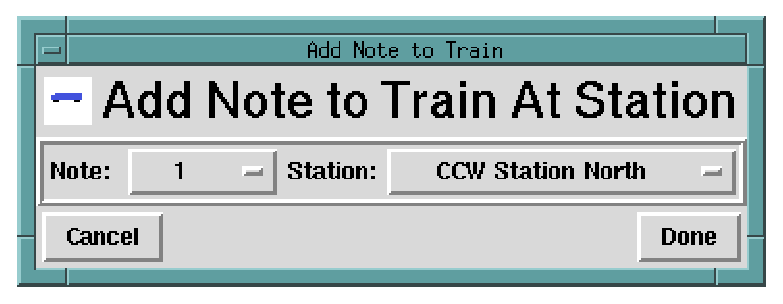
\epsfig{file=TimeTable/addNoteToTrainAtStation2.ps}\\
\caption{Add Note To Train at Station second dialog box.} 
\label{fig:addNoteToTrainAtStation2}
\end{centering} 
\end{figure}

\section{Remove Note From Train item} 

The ``Remove Note From Train'' menu item removes a note from a train.
The ``Remove Note From Train'' dialog box is displayed, as shown in
Figure~\ref{fig:removeNoteFromTrain}.

\begin{figure}
\begin{centering}
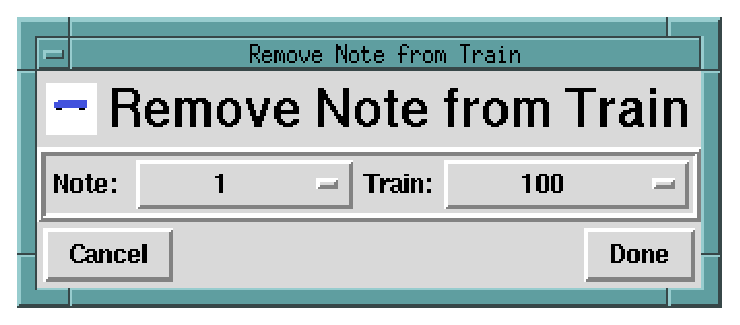
\epsfig{file=TimeTable/removeNoteFromTrain.ps}\\
\caption{Remove Note From Train dialog box.}
\label{fig:removeNoteFromTrain}
\end{centering}
\end{figure}

\section{Remove Note From Train at Station item}

The ``Remove Note From Train at Station'' menu item removes a note from
a train at a specific station. The ``Remove Note From Train at
Station'' dialog boxes are displayed, as shown in
Figures~\ref{fig:removeNoteFromTrainAtStation1} and
\ref{fig:removeNoteFromTrainAtStation2}.

\begin{figure} 
\begin{centering} 
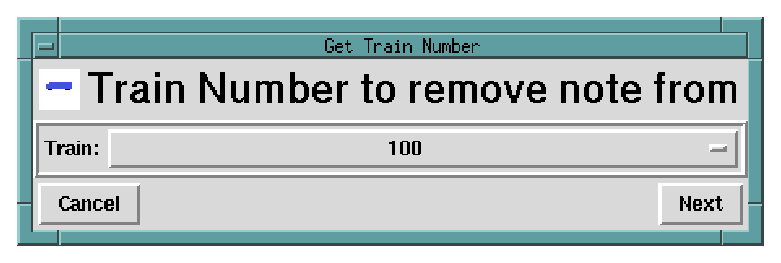
\epsfig{file=TimeTable/removeNoteFromTrainAtStation1.ps}\\
\caption{Remove Note From Train at Station first dialog box.} 
\label{fig:removeNoteFromTrainAtStation1}
\end{centering} 
\end{figure}

\begin{figure} 
\begin{centering} 
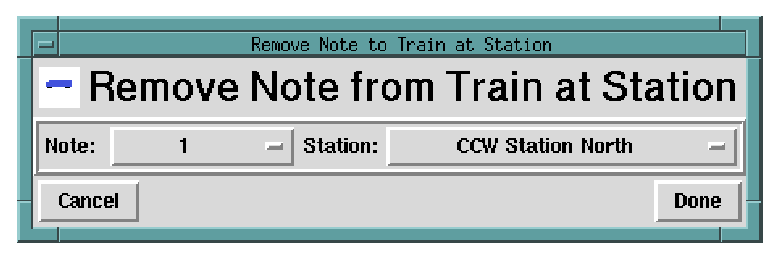
\epsfig{file=TimeTable/removeNoteFromTrainAtStation2.ps}\\
\caption{Remove Note From Train at Station second dialog box.} 
\label{fig:removeNoteFromTrainAtStation2}
\end{centering} 
\end{figure}


